\appendix
\section*{Appendices}
\addcontentsline{toc}{section}{Appendices}
\renewcommand{\thesubsection}{\Alph{subsection}}

\subsection{Bibliography}
\label{sec:Bibliography}

Engineering Industries Association. EIA Standard - EIA-274-D, Interchangeable Variable, Block Data Format for Positioning, Contouring, and Contouring/Positioning Numerically Controlled Machines. Washington, D.C. 1979.

ISO TC 184/SC4/WG3 N1089. ISO/DIS 10303-238: Industrial automation systems and integration  Product data representation and exchange  Part 238: Application Protocols: Application interpreted model for computerized numerical controllers. Geneva, Switzerland, 2004.

International Organization for Standardization. ISO 14649: Industrial automation systems and integration – Physical device control – Data model for computerized numerical controllers – Part 10: General process data. Geneva, Switzerland, 2004.

International Organization for Standardization. ISO 14649: Industrial automation systems and integration – Physical device control – Data model for computerized numerical controllers – Part 11: Process data for milling. Geneva, Switzerland, 2000.

International Organization for Standardization. ISO 6983/1 – Numerical Control of machines – Program format and definition of address words – Part 1: Data format for positioning, line and contouring control systems. Geneva, Switzerland, 1982.

Electronic Industries Association. ANSI/EIA-494-B-1992, 32 Bit Binary CL (BCL) and 7 Bit ASCII CL (ACL) Exchange Input Format for Numerically Controlled Machines. Washington, D.C. 1992.

National Aerospace Standard. Uniform Cutting Tests - NAS Series: Metal Cutting Equipment Specifications. Washington, D.C. 1969.

International Organization for Standardization. ISO 10303-11: 1994, Industrial automation systems and integration  Product data representation and exchange  Part 11: Description methods: The EXPRESS language reference manual. Geneva, Switzerland, 1994.

International Organization for Standardization. ISO 10303-21: 1996, Industrial automation systems and integration -- Product data representation and exchange -- Part 21: Implementation methods: Clear text encoding of the exchange structure. Geneva, Switzerland, 1996.

H.L. Horton, F.D. Jones, and E. Oberg. Machinery's Handbook. Industrial Press, Inc. New York, 1984.

International Organization for Standardization. ISO 841-2001: Industrial automation systems and integration - Numerical control of machines - Coordinate systems and motion nomenclature. Geneva, Switzerland, 2001.

ASME B5.57: Methods for Performance Evaluation of Computer Numerically Controlled Lathes and Turning Centers, 1998.

ASME/ANSI B5.54: Methods for Performance Evaluation of Computer Numerically Controlled Machining Centers. 2005.

OPC Foundation. OPC Unified Architecture Specification, Part 1: Concepts Version 1.00. July 28, 2006.

IEEE STD 1451.0-2007, Standard for a Smart Transducer Interface for Sensors and Actuators – Common Functions, Communication Protocols, and Transducer Electronic Data Sheet (TEDS) Formats, IEEE Instrumentation and Measurement Society, TC-9, The Institute of Electrical and Electronics Engineers, Inc., New York, N.Y. 10016, SH99684, October 5, 2007.

IEEE STD 1451.4-1994, Standard for a Smart Transducer Interface for Sensors and Actuators – Mixed-Mode Communication Protocols and Transducer Electronic Data Sheet (TEDS) Formats, IEEE Instrumentation and Measurement Society, TC-9, The Institute of Electrical and Electronics Engineers, Inc., New York, N.Y. 10016, SH95225, December 15, 2004. \newpage

\subsection{XML Schema Diagrams}
\label{sec:XML Schema Diagrams}

\subsubsection{Assets Schema Diagrams}
\label{sec:Assets Schema Diagrams}

\begin{figure}[ht]
  \centering
    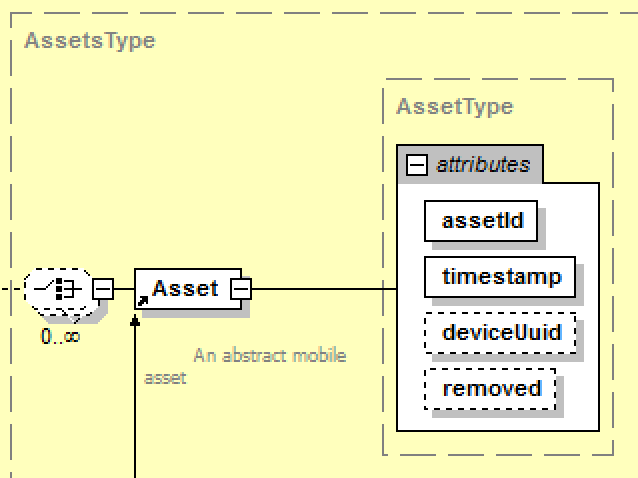
\includegraphics[width=1.0\textwidth]{figures/Asset Schema.png}
  \caption{Asset Schema Diagram}
  \label{fig:Asset Schema Diagram}
\end{figure}

\FloatBarrier


\begin{figure}[ht]
  \centering
    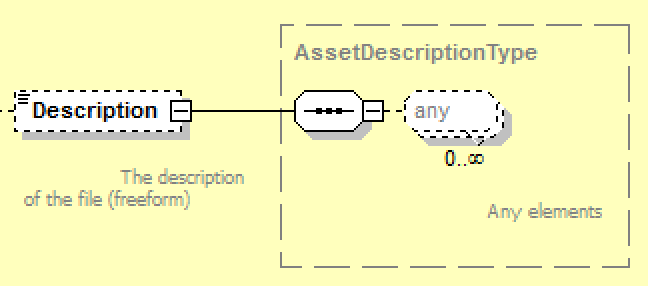
\includegraphics[width=1.0\textwidth]{figures/Description Schema.png}
  \caption{Description Schema Diagram}
  \label{fig:Description Schema Diagram}
\end{figure}

\FloatBarrier


\subsubsection{CuttingTool Schema Diagrams}
\label{sec:CuttingTool Schema Diagrams}

\begin{figure}[ht]
  \centering
    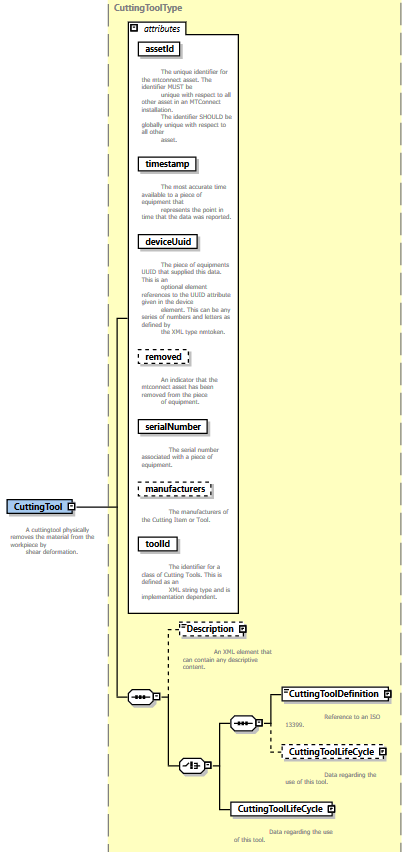
\includegraphics[width=1.0\textwidth]{figures/CuttingTool Schema.png}
  \caption{CuttingTool Schema Diagram}
  \label{fig:CuttingTool Schema Diagram}
\end{figure}

\FloatBarrier


\begin{figure}[ht]
  \centering
    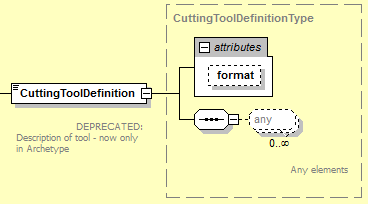
\includegraphics[width=1.0\textwidth]{figures/CuttingToolDefinition Schema.png}
  \caption{CuttingToolDefinition Schema Diagram}
  \label{fig:CuttingToolDefinition Schema Diagram}
\end{figure}

\FloatBarrier


\begin{figure}[ht]
  \centering
    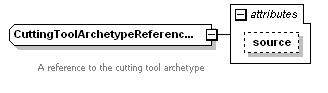
\includegraphics[width=1.0\textwidth]{figures/CuttingToolArchetypeReference Schema.png}
  \caption{CuttingToolArchetypeReference Schema Diagram}
  \label{fig:CuttingToolArchetypeReference Schema Diagram}
\end{figure}

\FloatBarrier


\subsubsection{CuttingToolLifeCycle Schema Diagrams}
\label{sec:CuttingToolLifeCycle Schema Diagrams}

\begin{figure}[ht]
  \centering
    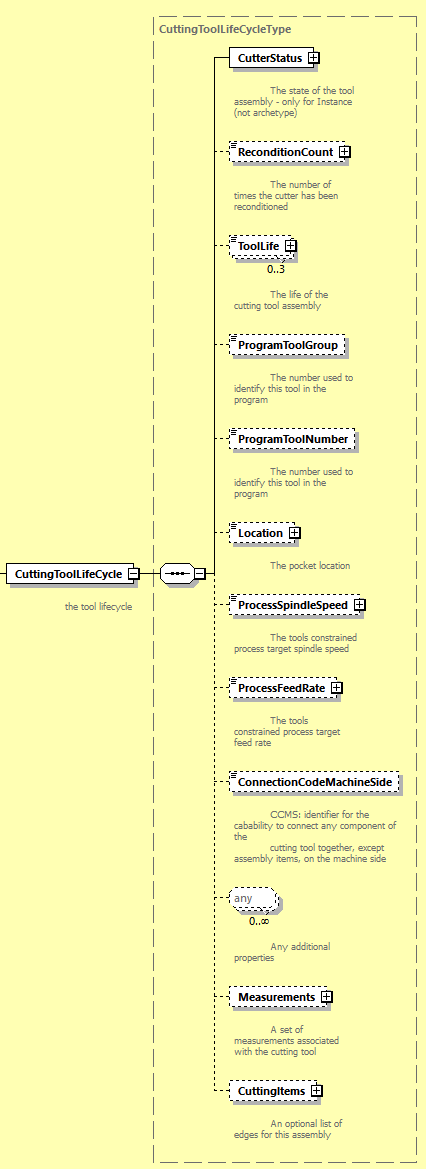
\includegraphics[width=1.0\textwidth]{figures/CuttingToolLifeCycle Schema.png}
  \caption{CuttingToolLifeCycle Schema Diagram}
  \label{fig:CuttingToolLifeCycle Schema Diagram}
\end{figure}

\FloatBarrier


\begin{figure}[ht]
  \centering
    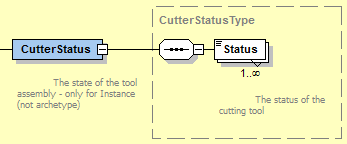
\includegraphics[width=1.0\textwidth]{figures/CutterStatus Schema.png}
  \caption{CutterStatus Schema Diagram}
  \label{fig:CutterStatus Schema Diagram}
\end{figure}

\FloatBarrier


\begin{figure}[ht]
  \centering
    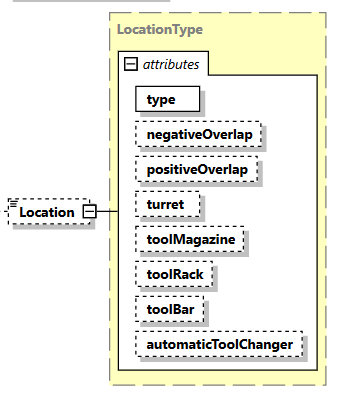
\includegraphics[width=1.0\textwidth]{figures/Location Schema.png}
  \caption{Location Schema Diagram}
  \label{fig:Location Schema Diagram}
\end{figure}

\FloatBarrier


\begin{figure}[ht]
  \centering
    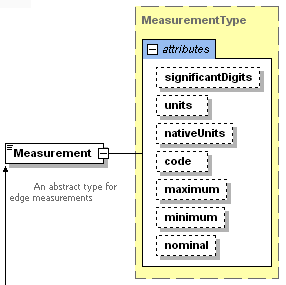
\includegraphics[width=1.0\textwidth]{figures/Measurement Schema.png}
  \caption{Measurement Schema Diagram}
  \label{fig:Measurement Schema Diagram}
\end{figure}

\FloatBarrier


\begin{figure}[ht]
  \centering
    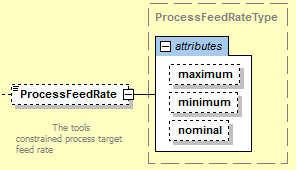
\includegraphics[width=1.0\textwidth]{figures/ProcessFeedRate Schema.png}
  \caption{ProcessFeedRate Schema Diagram}
  \label{fig:ProcessFeedRate Schema Diagram}
\end{figure}

\FloatBarrier


\begin{figure}[ht]
  \centering
    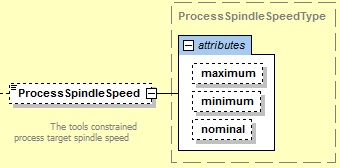
\includegraphics[width=1.0\textwidth]{figures/ProcessSpindleSpeed Schema.png}
  \caption{ProcessSpindleSpeed Schema Diagram}
  \label{fig:ProcessSpindleSpeed Schema Diagram}
\end{figure}

\FloatBarrier


\begin{figure}[ht]
  \centering
    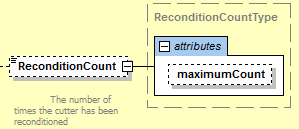
\includegraphics[width=1.0\textwidth]{figures/ReconditionCount Schema.png}
  \caption{ReconditionCount Schema Diagram}
  \label{fig:ReconditionCount Schema Diagram}
\end{figure}

\FloatBarrier


\begin{figure}[ht]
  \centering
    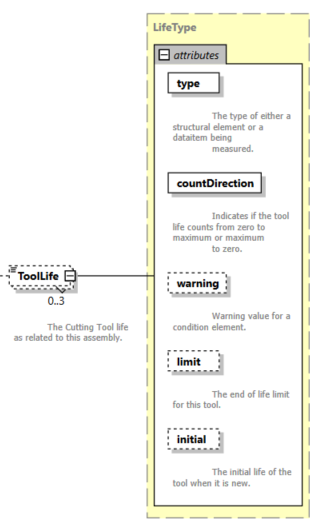
\includegraphics[width=1.0\textwidth]{figures/ToolLife Schema.png}
  \caption{ToolLife Schema Diagram}
  \label{fig:ToolLife Schema Diagram}
\end{figure}

\FloatBarrier


\subsubsection{CuttingItem Schema Diagrams}
\label{sec:CuttingItem Schema Diagrams}

\begin{figure}[ht]
  \centering
    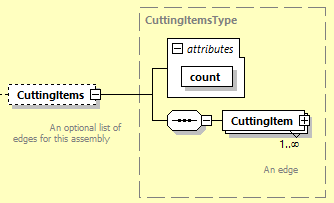
\includegraphics[width=1.0\textwidth]{figures/CuttingItems Schema.png}
  \caption{CuttingItems Schema Diagram}
  \label{fig:CuttingItems Schema Diagram}
\end{figure}

\FloatBarrier


\begin{figure}[ht]
  \centering
    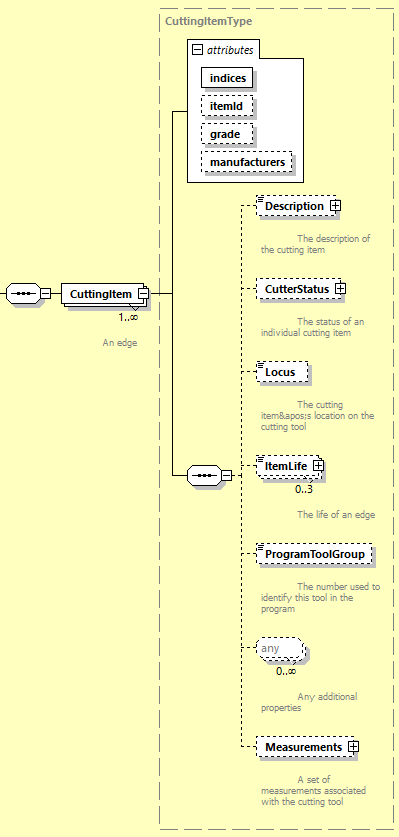
\includegraphics[width=1.0\textwidth]{figures/CuttingItem Schema.png}
  \caption{CuttingItem Schema Diagram}
  \label{fig:CuttingItem Schema Diagram}
\end{figure}

\FloatBarrier


\begin{figure}[ht]
  \centering
    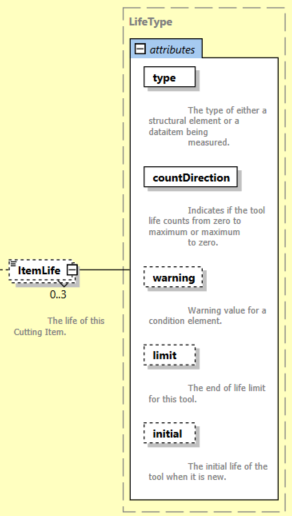
\includegraphics[width=1.0\textwidth]{figures/ItemLife Schema.png}
  \caption{ItemLife Schema Diagram}
  \label{fig:ItemLife Schema Diagram}
\end{figure}

\FloatBarrier


\subsubsection{ISO 13399 Diagrams}
\label{sec:ISO 13399 Diagrams}

\paragraph{Measurement Diagrams}
\label{sec:Measurement Diagrams}

\begin{figure}[ht]
  \centering
    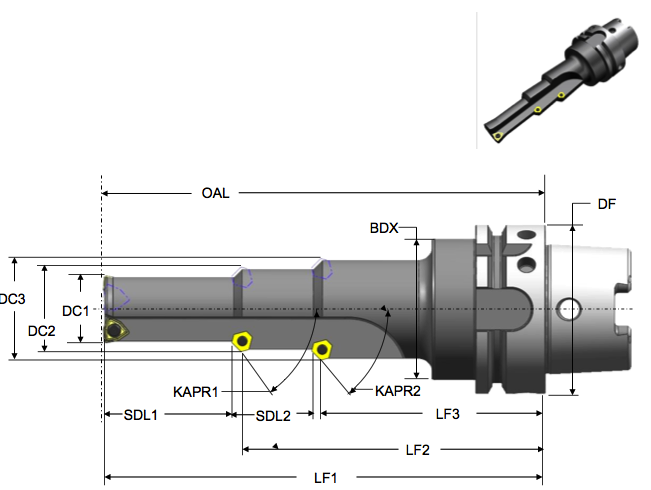
\includegraphics[width=1.0\textwidth]{figures/Cutting Tool Measurement 3.png}
  \caption{Cutting Tool Measurement 3 Diagram}
  \label{fig:Cutting Tool Measurement 3 Diagram}
\end{figure}

\FloatBarrier


\begin{figure}[ht]
  \centering
    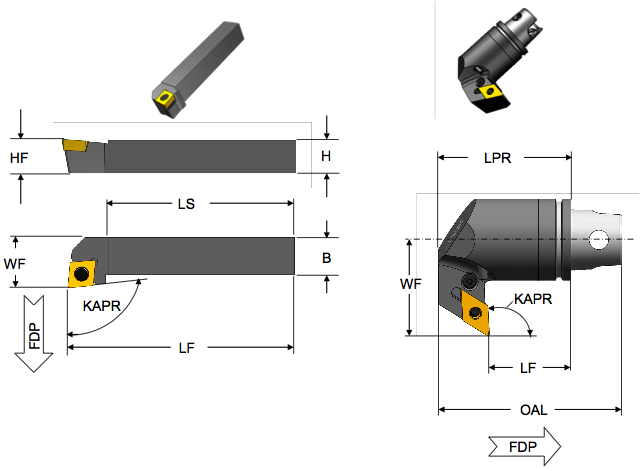
\includegraphics[width=1.0\textwidth]{figures/Cutting Tool Measurement 4.png}
  \caption{Cutting Tool Measurement 4 Diagram}
  \label{fig:Cutting Tool Measurement 4 Diagram}
\end{figure}

\FloatBarrier


\begin{figure}[ht]
  \centering
    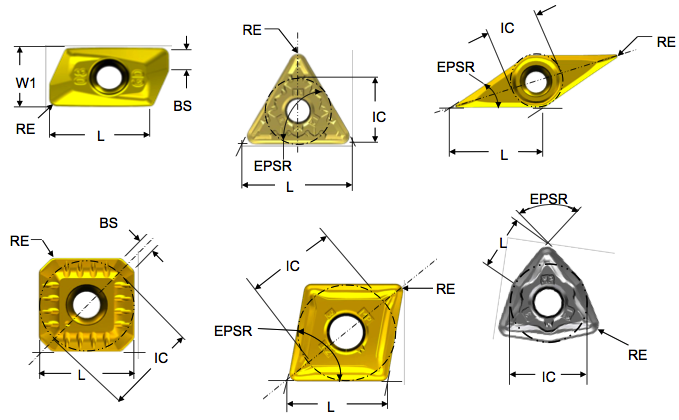
\includegraphics[width=1.0\textwidth]{figures/Cutting Tool Measurement 5.png}
  \caption{Cutting Tool Measurement 5 Diagram}
  \label{fig:Cutting Tool Measurement 5 Diagram}
\end{figure}

\FloatBarrier


\begin{figure}[ht]
  \centering
    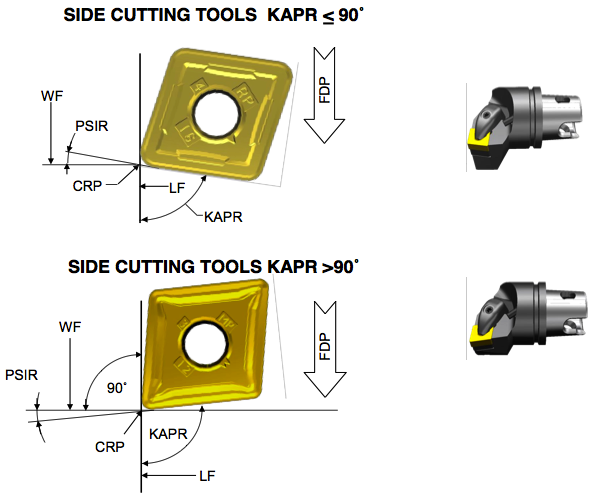
\includegraphics[width=1.0\textwidth]{figures/Cutting Tool Measurement 6.png}
  \caption{Cutting Tool Measurement 6 Diagram}
  \label{fig:Cutting Tool Measurement 6 Diagram}
\end{figure}

\FloatBarrier


\begin{figure}[ht]
  \centering
    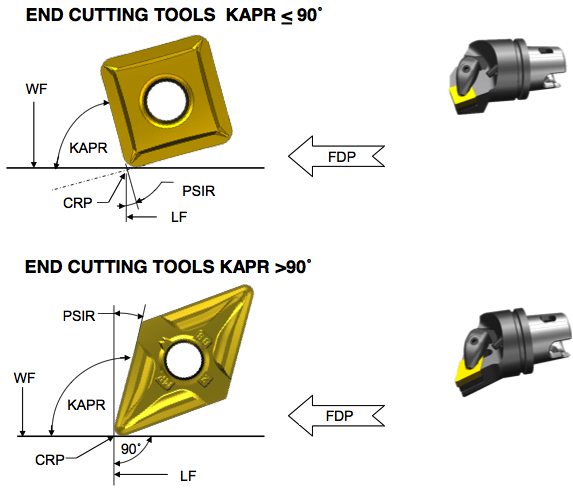
\includegraphics[width=1.0\textwidth]{figures/Cutting Tool Measurement 7.png}
  \caption{Cutting Tool Measurement 7 Diagram}
  \label{fig:Cutting Tool Measurement 7 Diagram}
\end{figure}

\FloatBarrier


\begin{figure}[ht]
  \centering
    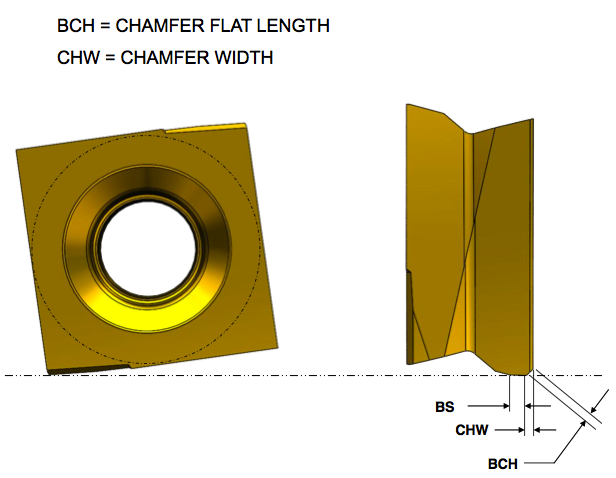
\includegraphics[width=1.0\textwidth]{figures/Cutting Tool Measurement 8.png}
  \caption{Cutting Tool Measurement 8 Diagram}
  \label{fig:Cutting Tool Measurement 8 Diagram}
\end{figure}

\FloatBarrier


\subsubsection{Cutting Tool Examples}}
\label{sec:Cutting Tool Examples}}

\paragraph{Shell Mill}}
\label{sec:Shell Mill}}

\begin{figure}[ht]
  \centering
    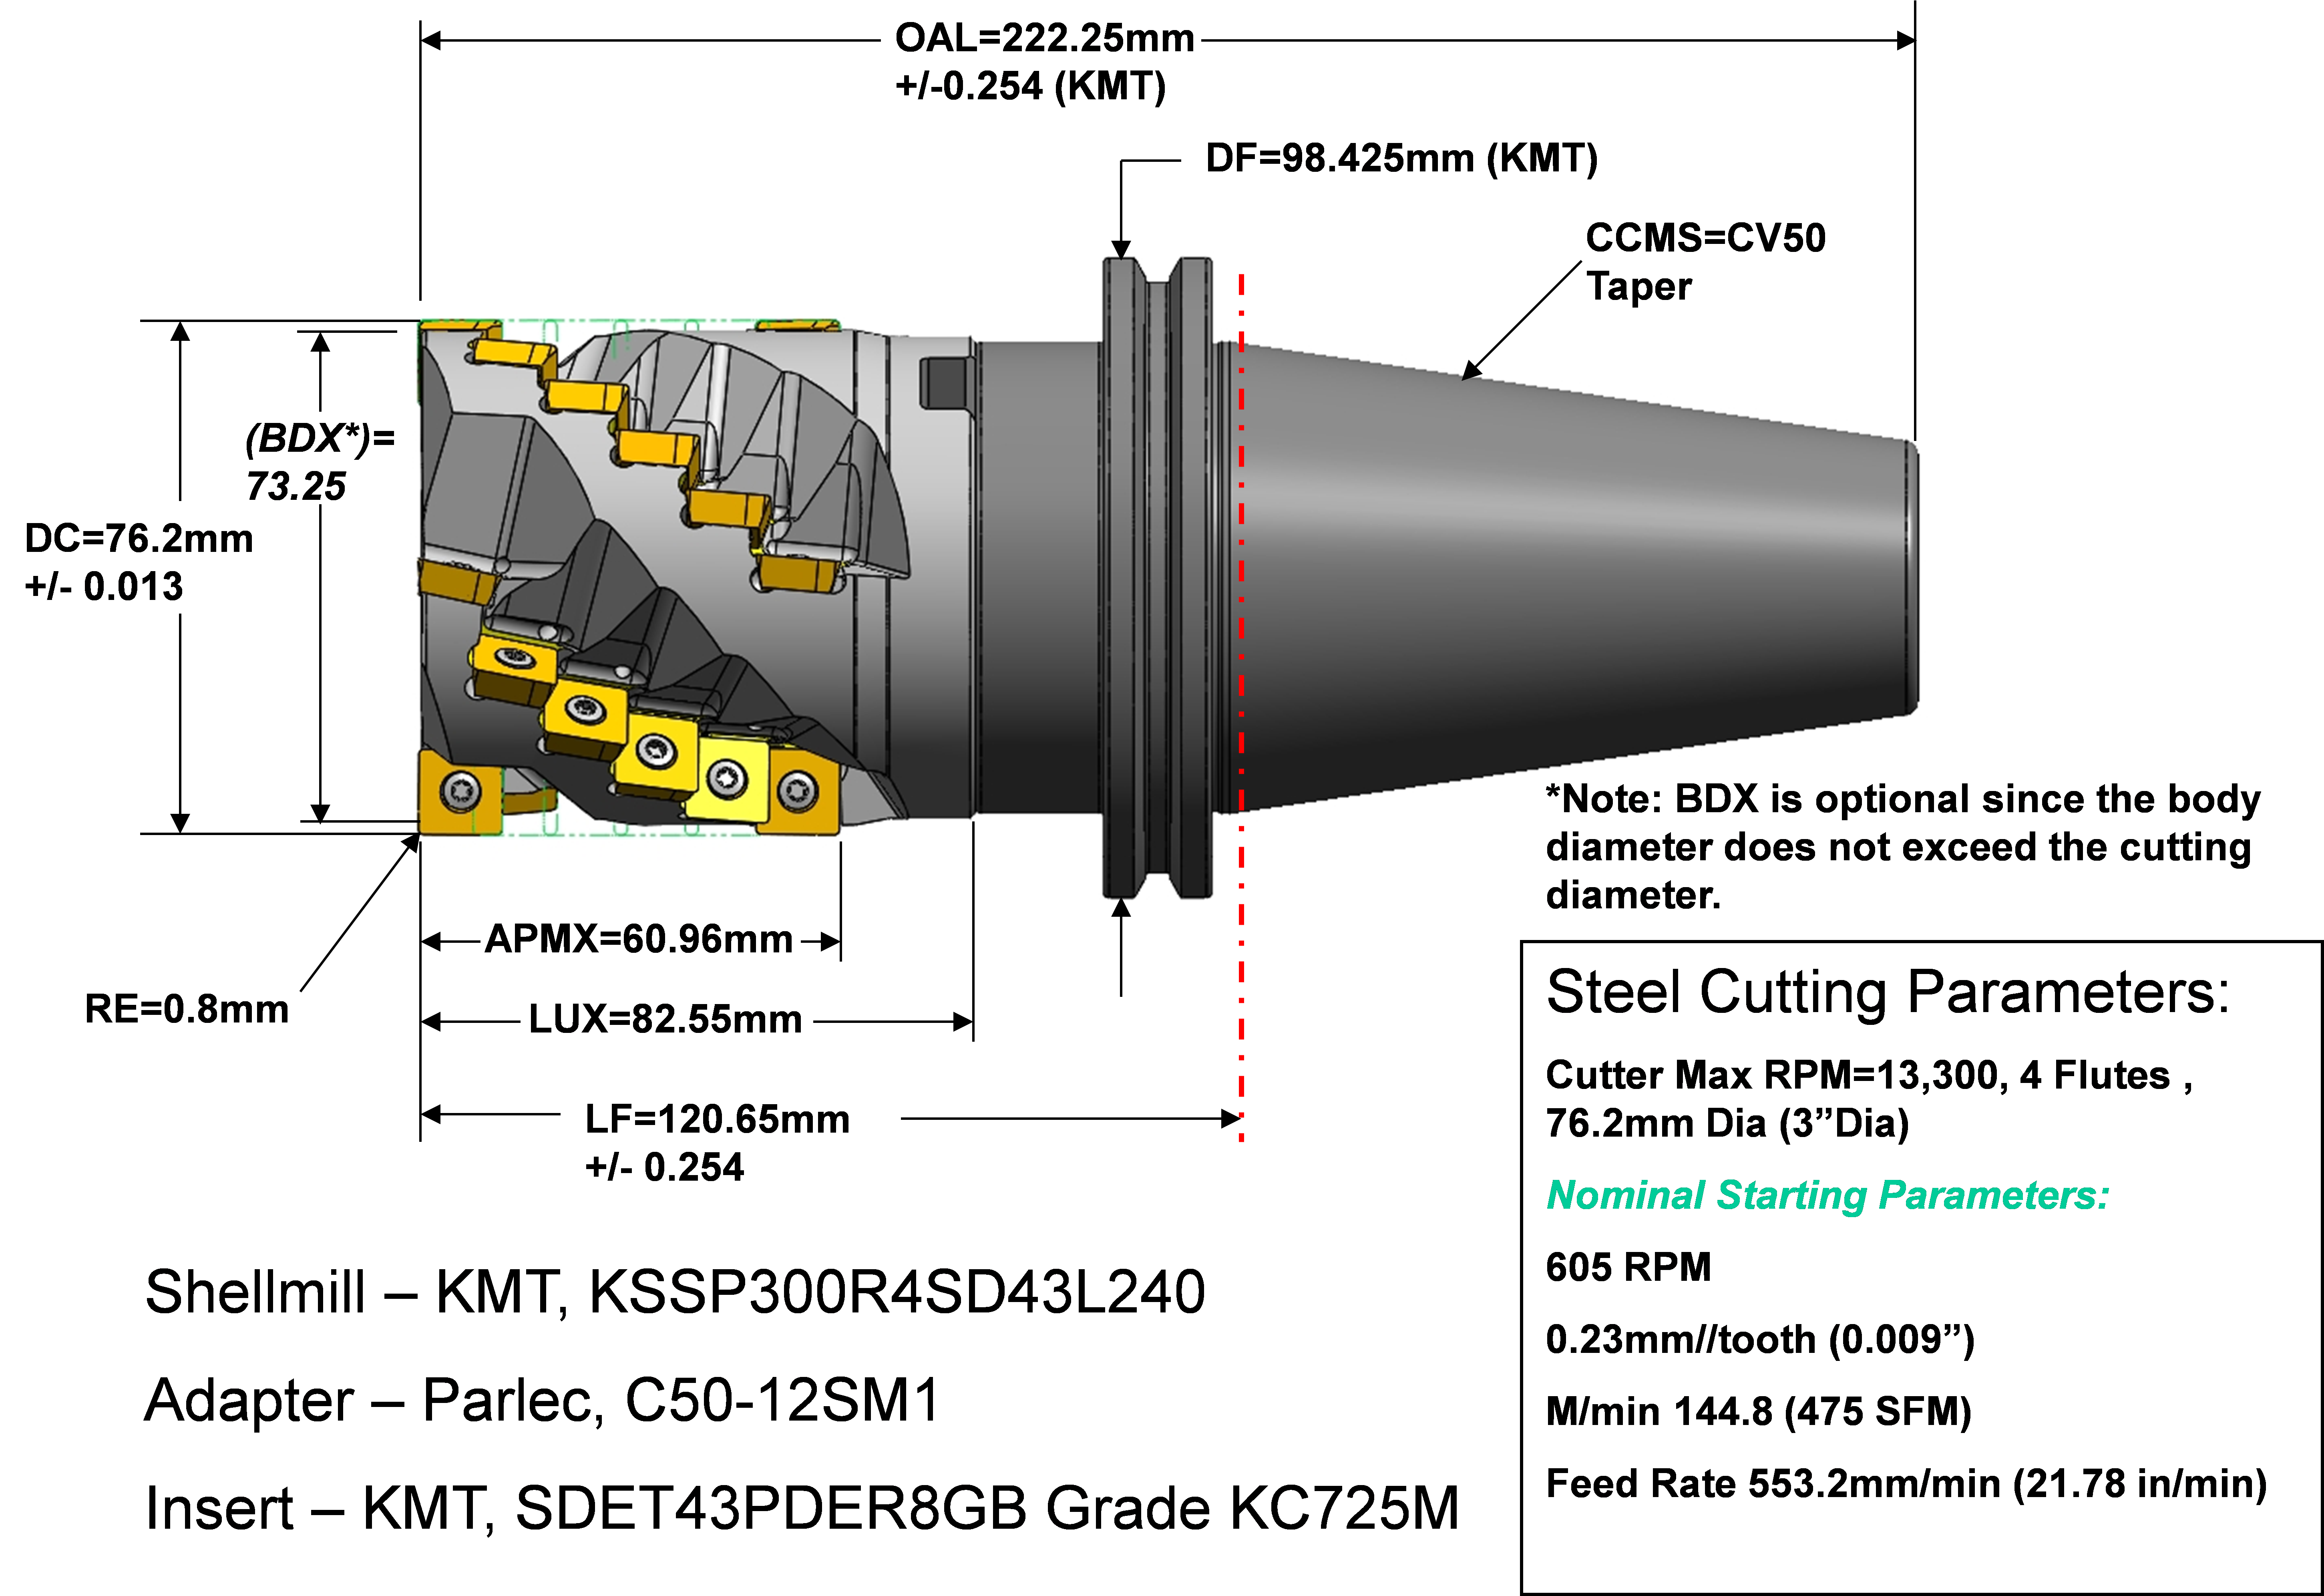
\includegraphics[width=1.0\textwidth]{figures/Shell Mill Side View.png}
  \caption{Shell Mill Side View Diagram}
  \label{fig:Shell Mill Side View Diagram}
\end{figure}

\FloatBarrier


\begin{figure}[ht]
  \centering
    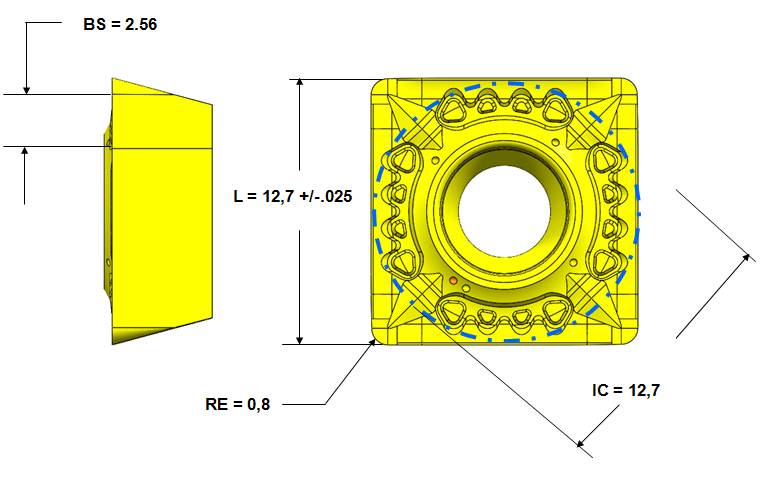
\includegraphics[width=1.0\textwidth]{figures/Indexable Insert Measurements.png}
  \caption{Indexable Insert Measurements Diagram}
  \label{fig:Indexable Insert Measurements Diagram}
\end{figure}

\FloatBarrier


	\begin{lstlisting}[firstnumber=1,escapechar=|,% 
	caption={Example for Indexable Insert Measurements}, label={lst:Example for Indexable Insert Measurements}]
	
<?xml version="1.0" encoding="UTF-8"?>
<MTConnectAssets 
xmlns:m="urn:mtconnect.org:MTConnectAssets:1.2" 
xmlns="urn:mtconnect.org:MTConnectAssets:1.2" 
xmlns:xsi="http://www.w3.org/2001/XMLSchema-instance" 
xsi:schemaLocation="urn:mtconnect.org:MTConnectAssets:1.2
http://mtconnect.org/schemas/MTConnectAssets\\textunderscore 1.2.xsd">
  <Header creationTime="2011-05-11T13:55:22" 
  assetBufferSize="1024" sender="localhost"
  assetCount="2" version="1.2" instanceId="1234"/>
  <Assets>
  <CuttingTool serialNumber="1" toolId="KSSP300R4SD43L240" 
  timestamp="2011-05-11T13:55:22" assetId="KSSP300R4SD43L240.1" 
  manufacturers="KMT,Parlec">
    <CuttingToolLifeCycle>
    <CutterStatus><Status>NEW</Status></CutterStatus>
    <ProcessSpindleSpeed maximum="13300" 
    nominal="605">10000</ProcessSpindleSpeed>
    <ProcessFeedRate
    nominal="9.22">9.22</ProcessSpindleSpeed>
    <ConnectionCodeMachineSide>CV50
    </ConnectionCodeMachineSide>
    <Measurements>
      <BodyDiameterMax code="BDX">73.25
      </BodyDiameterMax>
      <OverallToolLength nominal="222.25" 
        minimum="221.996" maximum="222.504" 
        code="OAL">222.25</OverallToolLength>
      <UsableLengthMax code="LUX" nominal="82.55">82.55
      </UsableLengthMax>
      <CuttingDiameterMax code="DC" nominal="76.2" 
        maximum="76.213" minimum="76.187">76.2
      </CuttingDiameterMax>
      <BodyLengthMax code="LF" nominal="120.65" 
        maximum="120.904" minimum="120.404">120.65
      </BodyLengthMax>
      <DepthOfCutMax code="APMX" 
      nominal="60.96">60.95</DepthOfCutMax>
      <FlangeDiameterMax code="DF" 
        nominal="98.425">98.425</FlangeDiameterMax>
    </Measurements>
    <CuttingItems count="24">
      <CuttingItem indices="1-24" itemId="SDET43PDER8GB" 
        manufacturers="KMT" grade="KC725M">
        <Measurements>
          <CuttingEdgeLength code="L" nominal="12.7" 
            minimum="12.675" maximum="12.725">12.7
          </CuttingEdgeLength>
        <WiperEdgeLength code="BS" nominal=
          "2.56">2.56</WiperEdgeLength>
        <IncribedCircleDiameter code="IC"
          nominal="12.7">12.7
        </IncribedCircleDiameter>
        <CornerRadius code="RE" nominal="0.8">
          0.8</CornerRadius>
      </Measurements>
      </CuttingItem>
    </CuttingItems>
    </CuttingToolLifeCycle>
    </CuttingTool>
  </Assets>
</MTConnectAssets>

	\end{lstlisting}


\pagebreak

\paragraph{Step Drill}
\label{sec:Step Drill}

\begin{figure}[ht]
  \centering
    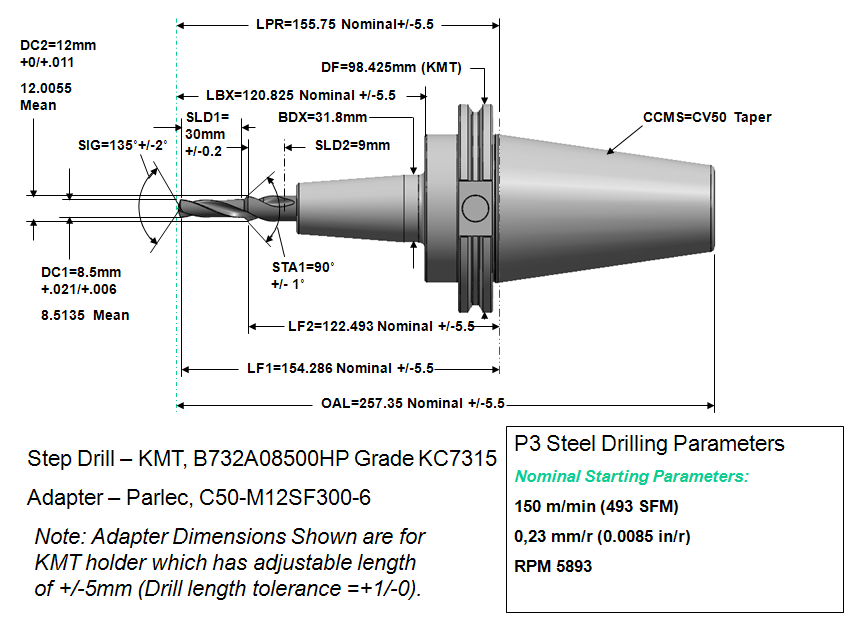
\includegraphics[width=1.0\textwidth]{figures/Step Mill Side View.png}
  \caption{Step Mill Side View Diagram}
  \label{fig:Step Mill Side View Diagram}
\end{figure}

\FloatBarrier


	\begin{lstlisting}[firstnumber=1,escapechar=|,% 
	caption={Example for Step Mill Side View}, label={lst:Example for Step Mill Side View}]
	
<?xml version="1.0" encoding="UTF-8"?>
<MTConnectAssets xmlns:m="urn:mtconnect.org:MTConnectAssets:1.2" 
xmlns="urn:mtconnect.org:MTConnectAssets:1.2" 
xmlns:xsi="http://www.w3.org/2001/XMLSchema-instance" 
xsi:schemaLocation="urn:mtconnect.org:MTConnectAssets:1.2 
http://mtconnect.org/schemas/MTConnectAssets\\textunderscore 1.2.xsd">
  <Header creationTime="2011-05-
  11T13:55:22" assetBufferSize="1024" 
  sender="localhost" assetCount="2" version="1.2" instanceId="1234"/>
  <Assets>
    <CuttingTool serialNumber="1 " toolId="B732A08500HP" 
    timestamp="2011-05-11T13:55:22" assetId="B732A08500HP " 
    manufacturers="KMT,Parlec">
      <Description>
        Step Drill - KMT, B732A08500HP Grade KC7315
        Adapter - Parlec, C50-M12SF300-6
      </Description>
      <CuttingToolLifeCycle>
        <CutterStatus><Status>NEW</Status></CutterStatus>
        <ProcessSpindleSpeed nominal="5893">5893</ProcessSpindleSpeed>
        <ProcessFeedRate nominal="2.5">2.5</ProcessFeedRate>
        <ConnectionCodeMachineSide>CV50 Taper</ConnectionCodeMachineSide>
        <Measurements>
          <BodyDiameterMax code="BDX">31.8</BodyDiameterMax>
          <BodyLengthMax code="LBX" nominal="120.825" maximum="126.325" 
          minimum="115.325">120.825</BodyLengthMax>
          <ProtrudingLength code="LPR" nominal="155.75" maximum="161.25" 
          minimum="150.26">155.75</ProtrudingLength>
          <FlangeDiameterMax code="DF" 
          nominal="98.425">98.425</FlangeDiameterMax>
          <OverallToolLength nominal="257.35" minimum="251.85" 
          maximum="262.85" code="OAL">257.35</OverallToolLength>
        </Measurements>
        <CuttingItems count="2">
          <CuttingItem indices="1" manufacturers="KMT" grade="KC7315">>
            <Measurements>
              <CuttingDiameter code="DC1" nominal="8.5" maximum="8.521" 
              minimum="8.506">8.5135</CuttingDiameter>
              <StepIncludedAngle code="STA1" nominal="90" maximum="91" 
              minimum="89">90</StepIncludedAngle>
              <FunctionalLength code="LF1" nominal="154.286" 
              minimum="148.786" 
              maximum="159.786">154.286</FunctionalLength>
              <StepDiameterLength code="SDL1" 
              nominal="9">9</StepDiameterLength>
              <PointAngle code="SIG" nominal="135" minimum="133" 
              maximum="137">135</PointAngle>
            </Measurements>
          </CuttingItem>
          <CuttingItem indices="2" manufacturers="KMT" grade="KC7315">>
            <Measurements>
              <CuttingDiameter code="DC2" nominal="12" maximum="12.011" 
              minimum="12">12</CuttingDiameter>
              <FunctionalLength code="LF2" nominal="122.493" 
              maximum="127.993" 
              minimum="116.993">122.493</FunctionalLength>
              <StepDiameterLength code="SDL2" 
              nominal="9">9</StepDiameterLength>
            </Measurements>
          </CuttingItem>
        </CuttingItems>
      </CuttingToolLifeCycle>
    </CuttingTool>
  </Assets>
</MTConnectAssets>

	\end{lstlisting}


\pagebreak

\paragraph{Shell Mill with Individual Loci}
\label{sec:Shell Mill with Individual Loci}

\begin{figure}[ht]
  \centering
    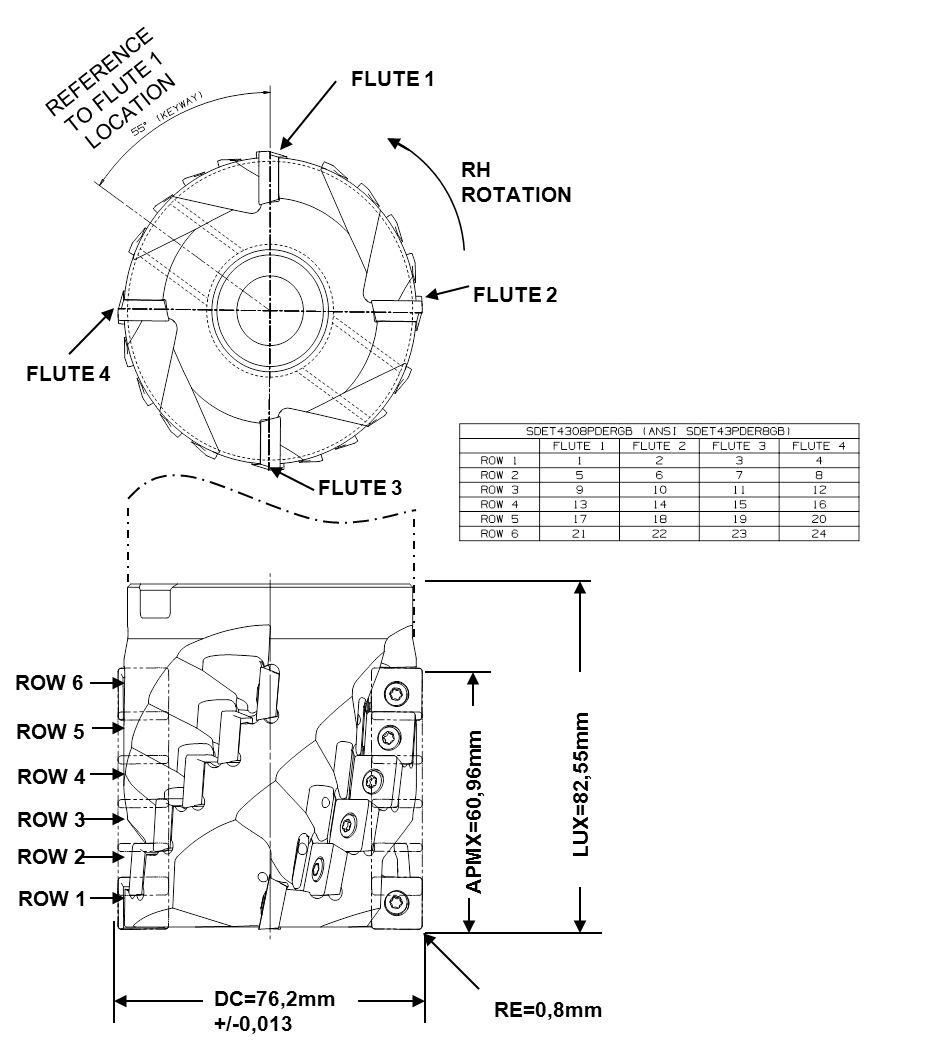
\includegraphics[width=1.0\textwidth]{figures/Shell Mill with Explicate Loci.png}
  \caption{Shell Mill with Explicate Loci Diagram}
  \label{fig:Shell Mill with Explicate Loci Diagram}
\end{figure}

\FloatBarrier


	\begin{lstlisting}[firstnumber=1,escapechar=|,% 
	caption={Example for Shell Mill with Explicate Loci}, label={lst:Example for Shell Mill with Explicate Loci}]
	
<?xml version="1.0" encoding="UTF-8"?>
<MTConnectAssets xmlns:m="urn:mtconnect.org:MTConnectAssets:1.2" 
xmlns="urn:mtconnect.org:MTConnectAssets:1.2" 
xmlns:xsi="http://www.w3.org/2001/XMLSchema-instance" 
xsi:schemaLocation="urn:mtconnect.org:MTConnectAssets:1.2 
http://mtconnect.org/schemas/MTConnectAssets\\textunderscore 1.2.xsd">
  <Header creationTime="2011-05-11T13:55:22" assetBufferSize="1024" 
  sender="localhost" assetCount="2" version="1.2" instanceId="1234"/>
  <Assets>
    <CuttingTool serialNumber="1" toolId="KSSP300R4SD43L240" 
    timestamp="2011-05-11T13:55:22" assetId="KSSP300R4SD43L240.1" 
    manufacturers="KMT,Parlec">
      <Description>Keyway: 55 degrees</Description>
      <CuttingToolLifeCycle>
        <CutterStatus><Status>NEW</Status></CutterStatus>
        <Measurements>
          <UsableLengthMax code="LUX" 
          nominal="82.55">82.55</UsableLengthMax>
          <CuttingDiameterMax code="DC" nominal="76.2" maximum="76.213" 
          minimum="76.187">76.2</CuttingDiameterMax>
          <DepthOfCutMax code="APMX" nominal="60.96">60.95</DepthOfCutMax>
        </Measurements>
        <CuttingItems count="24">
          <CuttingItem indices="1" itemId="SDET43PDER8GB" 
          manufacturers="KMT">
            <Locus>FLUTE: 1, ROW: 1</Locus>
            <Measurements>
             <DriveAngle code="DRVA" nominal="55">55</DriveAngle>
           </Measurements>
          </CuttingItem>
          <CuttingItem indices="2-24" itemId="SDET43PDER8GB" 
          manufacturers="KMT">
            <Locus>FLUTE: 2-4, ROW: 1; FLUTE: 1-4, ROW 2-6</Locus>
          </CuttingItem>
        </CuttingItems>
      </CuttingToolLifeCycle>
    </CuttingTool>
  </Assets>
</MTConnectAssets>

	\end{lstlisting}


\pagebreak

\paragraph{Drill with Individual Loci}
\label{sec:Drill with Individual Loci}

\begin{figure}[ht]
  \centering
    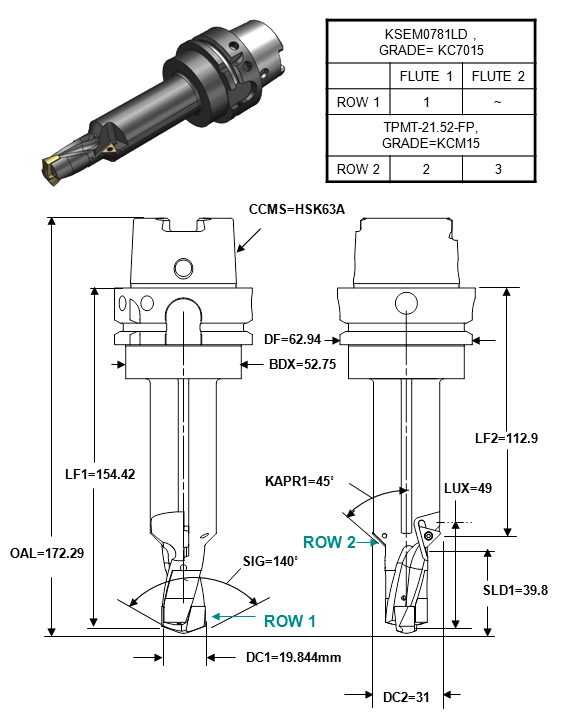
\includegraphics[width=1.0\textwidth]{figures/Step Drill with Explicate Loci.png}
  \caption{Step Drill with Explicate Loci Diagram}
  \label{fig:Step Drill with Explicate Loci Diagram}
\end{figure}

\FloatBarrier


	\begin{lstlisting}[firstnumber=1,escapechar=|,% 
	caption={Example for Step Drill with Explicate Loci}, label={lst:Example for Step Drill with Explicate Loci}]
	
<?xml version="1.0" encoding="UTF-8"?>
<MTConnectAssets xmlns:m="urn:mtconnect.org:MTConnectAssets:1.2" 
xmlns="urn:mtconnect.org:MTConnectAssets:1.2" 
xmlns:xsi="http://www.w3.org/2001/XMLSchema-instance" 
xsi:schemaLocation="urn:mtconnect.org:MTConnectAssets:1.2 
http://mtconnect.org/schemas/MTConnectAssets\\textunderscore 1.2.xsd">
  <Header creationTime="2011-05-11T13:55:22" assetBufferSize="1024" 
  sender="localhost" assetCount="2" version="1.2" instanceId="1234"/>
  <Assets>
    <CuttingTool serialNumber="1" toolId="KSEM0781LD" 
    timestamp="2011-05-11T13:55:22" assetId="KSEM0781LD.1" manufacturers="KMT">
      <CuttingToolLifeCycle>
        <CutterStatus><Status>NEW</Status></CutterStatus>
        <ConnectionCodeMachineSide>HSK63A</ConnectionCodeMachineSide>
        <Measurements>
          <BodyDiameterMax code="BDX">52.75</BodyDiameterMax>
          <OverallToolLength nominal="172.29" 
          code="OAL">172.29</OverallToolLength>
          <UsableLengthMax code="LUX" nominal="49">49</UsableLengthMax>
          <FlangeDiameterMax code="DF" 
          nominal="62.94">62.94</FlangeDiameterMax>
        </Measurements>
        <CuttingItems count="3">
          <CuttingItem indices="1" itemId="KSEM0781LD" manufacturers="KMT" 
          grade="KC7015">
            <Locus>FLUTE: 1, ROW: 1</Locus>
            <Measurements>
         <FunctionalLength code="LF1" nominal="154.42">154.42</FunctionalLength>
         <CuttingDiameter code="DC1" nominal="19.844">19.844</CuttingDiameter>
         <PointAngle code="SIG" nominal="140">140</PointAngle>
         <ToolCuttingEdgeAngle code="KAPR1" nominal="45">45</ToolCuttingEdgeAngle>
         <StepDiameterLength code="SLD1" nominal="39.8">39.8</StepDiameterLength>
            </Measurements>
          </CuttingItem>
          <CuttingItem indices="2-3" itemId="TPMT-21.52-FP" 
          manufacturers="KMT" grade="KCM15">
            <Locus>FLUTE: 1-2, ROW: 2</Locus>
            <Measurements>
         <FunctionalLength code="LF2" nominal="112.9">119.2</FunctionalLength>
         <CuttingDiameter code="DC2" nominal="31">31</CuttingDiameter>
            </Measurements>
          </CuttingItem>
        </CuttingItems>
      </CuttingToolLifeCycle>
    </CuttingTool>
  </Assets>
</MTConnectAssets>

	\end{lstlisting}


\pagebreak

\paragraph{Shell Mill with Different Inserts on First Row}
\label{sec:Shell Mill with Different Inserts on First Row}

\begin{figure}[ht]
  \centering
    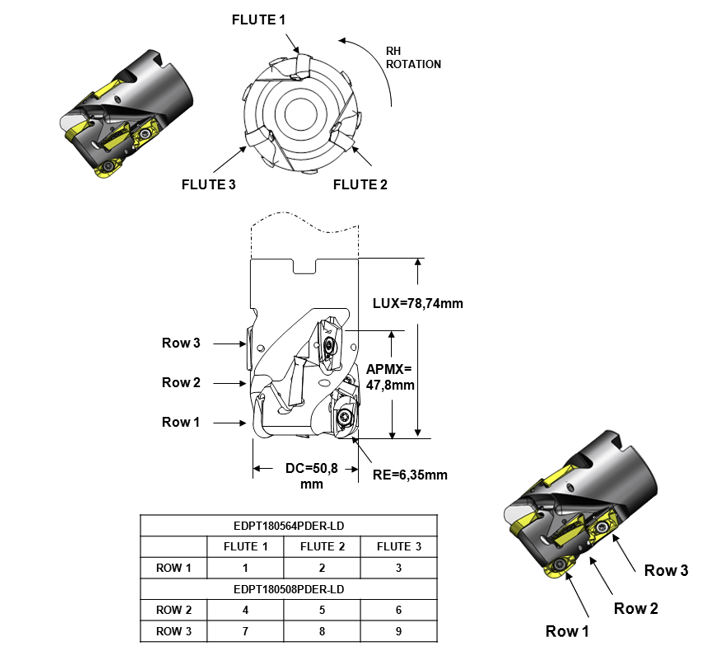
\includegraphics[width=1.0\textwidth]{figures/Shell Mill with Different Inserts on First Row.png}
  \caption{Shell Mill with Different Inserts on First Row Diagram}
  \label{fig:Shell Mill with Different Inserts on First Row Diagram}
\end{figure}

\FloatBarrier


	\begin{lstlisting}[firstnumber=1,escapechar=|,% 
	caption={Example for Shell Mill with Different Inserts on First Row}, label={lst:Example for Shell Mill with Different Inserts on First Row}]
	
<?xml version="1.0" encoding="UTF-8"?>
<MTConnectAssets xmlns:m="urn:mtconnect.org:MTConnectAssets:1.2" 
xmlns="urn:mtconnect.org:MTConnectAssets:1.2" 
xmlns:xsi="http://www.w3.org/2001/XMLSchema-instance" 
xsi:schemaLocation="urn:mtconnect.org:MTConnectAssets:1.2 
http://mtconnect.org/schemas/MTConnectAssets\\textunderscore 1.2.xsd">
  <Header creationTime="2011-05-11T13:55:22" assetBufferSize="1024" 
  sender="localhost" assetCount="2" version="1.2" instanceId="1234"/>
  <Assets>
    <CuttingTool serialNumber="1" toolId="XXX" timestamp="2011-05-11T13:55:22" 
    assetId="XXX.1" manufacturers="KMT">
      <CuttingToolLifeCycle>
        <CutterStatus><Status>NEW</Status></CutterStatus>
        <Measurements>
          <DepthOfCutMax code="APMX" nominal="47.8">47.8</DepthOfCutMax>
          <CuttingDiameterMax code="DC" 
          nominal="50.8">50.8</CuttingDiameterMax>
          <UsableLengthMax code="LUX" 
          nominal="78.74">78.74</UsableLengthMax>
        </Measurements>
        <CuttingItems count="9">
          <CuttingItem indices="1-3" itemId="EDPT180564PDER-LD" 
          manufacturers="KMT">
            <Locus>FLUTE: 1-3, ROW: 1</Locus>
            <Measurements>
              <CornerRadius code="RE" nominal="6.25">6.35</CornerRadius>
            </Measurements>
          </CuttingItem>
          <CuttingItem indices="4-9" itemId="EDPT180508PDER-LD" 
          manufacturers="KMT">
            <Locus>FLANGE: 1-4, ROW: 2-3</Locus>
          </CuttingItem>
        </CuttingItems>
      </CuttingToolLifeCycle>
    </CuttingTool>
  </Assets>
</MTConnectAssets>

	\end{lstlisting}



\subsubsection{File Schema Diagrams}
\label{sec:File Schema Diagrams}

\begin{figure}[ht]
  \centering
    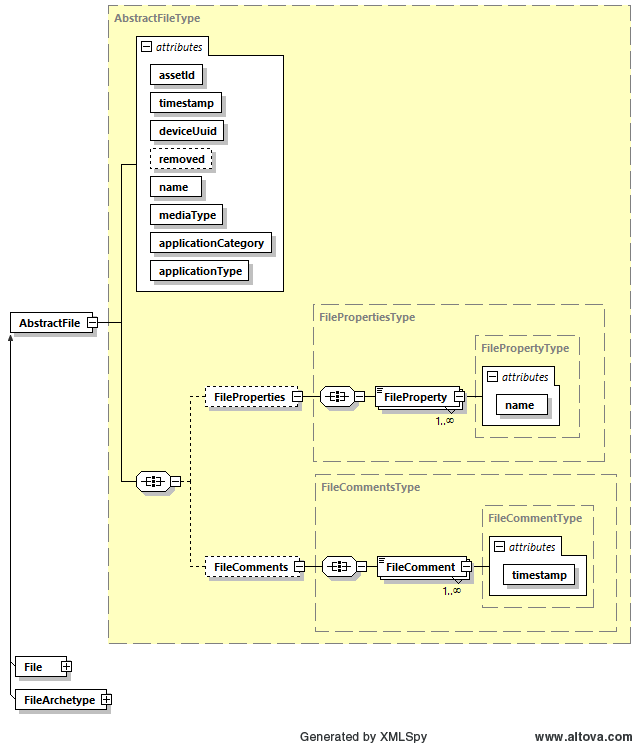
\includegraphics[width=1.0\textwidth]{figures/AbstractFile Schema.png}
  \caption{AbstractFile Schema Diagram}
  \label{fig:AbstractFile Schema Diagram}
\end{figure}

\FloatBarrier


\begin{figure}[ht]
  \centering
    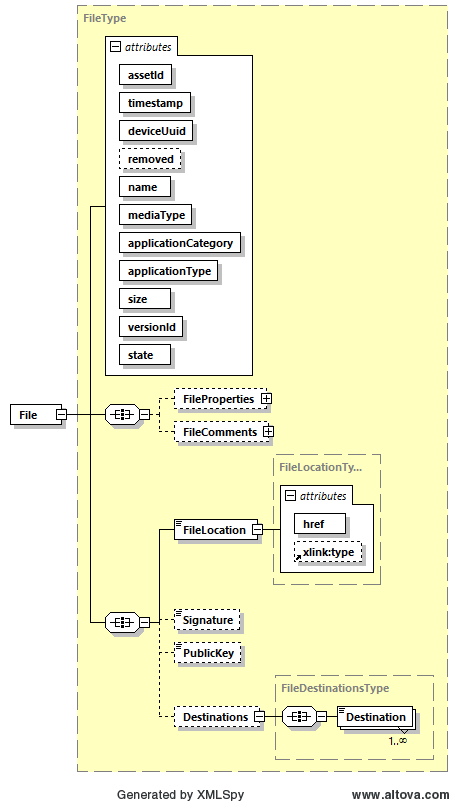
\includegraphics[width=1.0\textwidth]{figures/File Schema.png}
  \caption{File Schema Diagram}
  \label{fig:File Schema Diagram}
\end{figure}

\FloatBarrier
